\section*{Cara setting environtment}
 \begin{enumerate}
	\item klik kanan pada this pc lalu pilih properties
	\begin{figure} [h]
	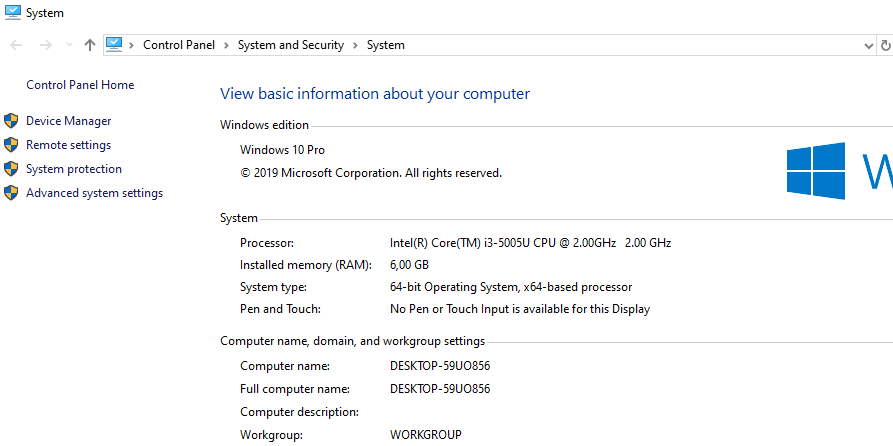
\includegraphics[width=9cm]{section/picpyt/env/env1.png}
	\centering
	\end{figure}
	
	 
	\item pilih advanced system settings
	\begin{figure} [h]
	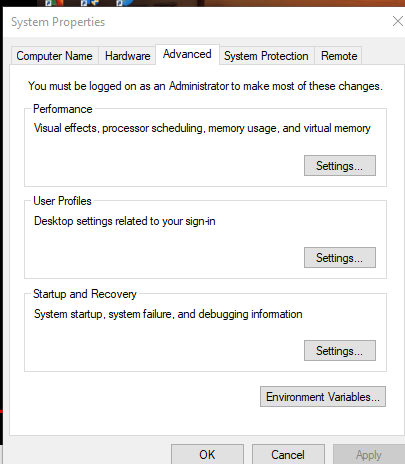
\includegraphics[width=7cm]{section/picpyt/env/env2.png}
	\centering
	\end{figure}
	
	\item pilih new dan buat seperti gambar dan variable value diisi dengan lokasi AppData python
	\begin{figure} [h]
	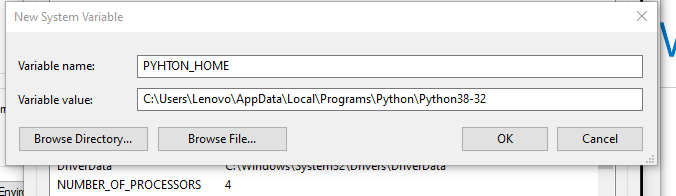
\includegraphics[width=10cm]{section/picpyt/env/env6.png}
	\centering
	\end{figure}
	
	\item cari Path. lalu edit dan isi dengan seperti berikut (urutan terakhir)
	\begin{figure} [h]
	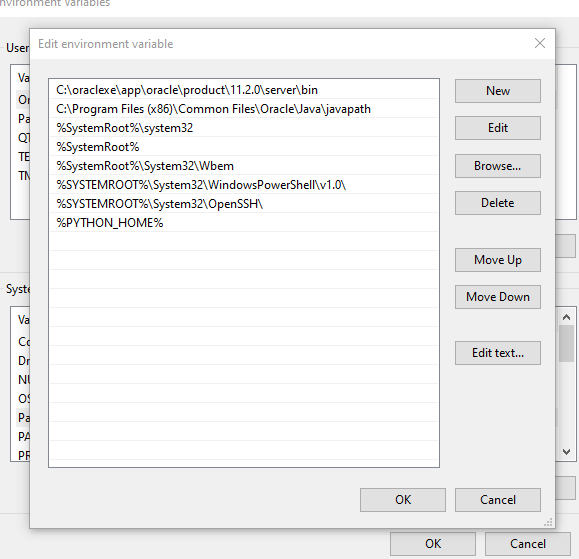
\includegraphics[width=7cm]{section/picpyt/env/env7.png}
	\centering
	\end{figure}
	
	\item buka cmd dan tulis python
	\begin{figure} [h]
	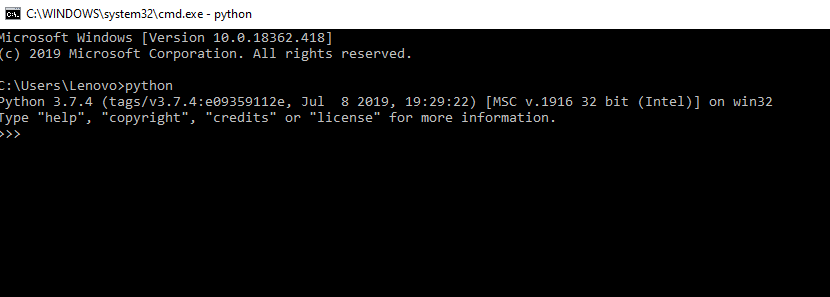
\includegraphics[width=7cm]{section/picpyt/env/env5.png}
	\centering
	\end{figure}
	
	\item maka setting environment sudah selesai
	
	
	
	
    \end{enumerate}



